\documentclass[12pt,a4paper,oneside]{ctexrep}
\setCJKmainfont{AR PL UKai CN}
\setCJKmonofont{AR PL UKai CN}
\usepackage{amsthm}
\usepackage{amsmath}
\usepackage[dvips]{graphicx}
\title{计算理论与函数式编程简介}
\author{曹竞帆}

\theoremstyle{definition}
\newtheorem{rf}{Primitive Recursion Function}
\newtheorem{con}[rf]{常数函数}
\newtheorem{suc}[rf]{后继函数}
\newtheorem{pro}[rf]{投影函数}
\newtheorem{com}[rf]{复合算子}
\newtheorem{pri}[rf]{原始递归算子}
\newtheorem{tm}{图灵机}

\begin{document}
\date{}
\maketitle

\begin{abstract}

本次课主要讨论两个部分的问题。

首先会从数理逻辑的角度讲解计算理论的发源。
通常我们提到计算机发源的时候首先想到的都是ENIAC,
但这是工程实践中的“第一个”。
科学技术的发展从来都是理论先行,那么计算机发源的理论根源在哪里呢?

第二部分我们会开始认识对函数式编程语言产生重要影响,
或者说就是函数式编程语言之理论根基的Lambda演算。
看看两条简单的公理是如何构造出一个完整的计算世界的。

%第三部分我们来看看函数式编程语言,思考与“传统”命令式编程语言在
%思维方式以及抽象思想上的异同。

%最后一部分,我们针对函数式编程语言中的Lisp家族进行剖析,
%感受Lisp的优点与不足之处。

%最后附上希尔伯特的一句话
\begin{quote}
``We must know---we will know!''
\end{quote}

\end{abstract}

\chapter{希尔伯特的梦}

\section{完备么?一致么?}

\subsection{第三次数学危机}

首先简单交代一下时代背景。
19世纪,伟大的德国数学家康托创立了现代集合论,
虽然没有立即受到其他数学家的认可(康托因此罹患抑郁症并于1918年在精神病院中去世)。
但这并没有阻止后来的数学家将集合论作为基础带入数学的形式化过程中来。
希尔伯特本人就曾经说过:“没有人能够把我们从康托建立的乐园中赶出去。”

然而,早在1897年,福尔蒂就揭示了集合论中的第一个悖论-----布拉利-福尔蒂悖论。

两年后,康托自己也发现了很相似的最大基数悖论。

1901年,罗素又提出了著名的罗素悖论。

由于此时,集合概念已经渗透到众多的数学分支,并且实际上集合论成了数学的基础,
因此集合论中一系列悖论的发现自然地引起了对数学的整个基本结构的有效性的怀疑。

史称“第三次数学危机”。

\subsection{希尔伯特计划}

大卫·希尔伯特,德国著名数学家,有人称其为“数学界最后一位全才”。
在经过多年在不同数学领域颇有建树地研究之后,希尔伯特将目光投向了整个数学,
他试图将数学建立在一个坚实的基础之上。
1928年,希尔伯特为了捍卫古典数学的尊严,避免悖论以解决数学最基础的问题,
提出了著名的“希尔伯特计划”。

这个计划的主要目标,是为全部的数学提供一个安全的理论基础。具体地,这个基础应该包括:
\begin{quote}
所有数学的形式化。意思是,所有数学应该用一种统一的严格形式化的语言,并且按照一套严格的规则来使用。

完备性。我们必须证明以下命题:在形式化之后,数学里所有的真命题都可以被证明(根据上述规则)。

一致性。我们必须证明:运用这一套形式化和它的规则,不可能推导出矛盾。

保守性。我们需要证明:如果某个关于“实际物”的结论用到了“假想物”(如不可数集合)来证明,那么不用“假想物”的话我们依然可以证明同样的结论。

判定性。应该有一个算法,来确定每一个形式化的命题是真命题还是假命题。
\end{quote}

\subsection{希尔伯特问题}

时间倒回到1900年。

那一年,在巴黎举行的第二届国际数学家大会上,
希尔伯特做了一次堪称数学史上影响最为深远的演讲,
演讲的题目叫做 “数学问题”。
在这一演讲中,希尔伯特列举了二十三个他认为最具重要意义的数学问题。
这些问题被后人称为 “希尔伯特问题”。
解决希尔伯特问题成了许多数学家终生奋斗的目标,
而在解决这些问题的过程中源源不断地产生出的成果则为二十世纪的数学发展注入了极大的生机\cite{tenth}。

其中第二个问题,算数公理系统的相容性问题,于1931年被哥德尔的不完备性定理解决。

随之而来的是希尔伯特计划的第二步无法实行,希尔伯特的梦破灭了。

理论上,哥德尔理论仍留下了一线希望:
也许可以给出一个算法判定一个给定的命题是否是不确定的,
让数学家可以忽略掉这些不确定的命题。

然而,1937年图灵发表他的论文《论可计算数及其在判定问题中的应用》,证明了不存在这样的算法,
希尔伯特计划的最后一步也是不可能的。

尽管这样,哥德尔的不完备性定理仍然带给我们很多教益。
至少我们知道了,有些东西我们不可能知道。
在哥德尔的这个划时代的证明之后,数学家对数学的基本工具-----证明-----有了新的认识。
专门研究数学证明的证明论,在他的启发下蓬勃发展。
但是,哥德尔教给我们最重要的一点是\cite{dream}:

\begin{quote}
数学,如同人生,如同爱情,有些东西是真的,你却永远无法证明。
\end{quote}

\section{可判定么?}

\subsection{可计算函数}

希尔伯特第十问题-----丢番图方程可解性问题-----以及后来的希尔伯特计划中的可判定性问题都促使
数学家们思考这样一个问题:

\begin{quote}
能否找到一种方法,仅仅通过机械化的计算,就能判定某个数学陈述是对是错?
也即数学证明能否机械化?
\end{quote}

因为哥德尔的工作已经证明数学在形式化中的本质缺陷,
数学家们将可判定性问题视为数学的“最后尊严”,并试图通过给出这个问题一个肯定的回答
来维护数学的崇高地位。

数学家们首先要做的是将“可计算”这个概念形式化。
因为要解决可判定问题,核心任务是要提出算法,十分明确毫不含糊的算法,
而算法是用来计算函数的,于是首先需要解决的问题是-----
什么是有效可计算的函数?也即算法可计算的函数?

虽然你可能非常惊讶,但我还是要说,递归函数在可计算理论中扮演核心问题的角色,
甚至在可计算理论发源的那个时期,计算理论不叫计算理论,就叫递归函数理论。
术语“递归的”是“可判定的”同义词,说一个问题是递归的,就是说:“这个问题足够
简单,可以用递归函数来解答这个问题,并且这个函数总是终止。”

递归在数学上首要的意义是“用归纳来定义”,或者说得绕口一点“用递归来定义”。
以我们目前的理解来非形式化地描述递归函数
就是说在一个函数$f$关于参数$x$的定义中需要用到之前的$f$的关于参数$y$的定义,或者说
在函数$f$的定义中需要用到已经定义的$g$函数。

为了简化讨论,接下来所出现的函数均定义在自然数集上。

\paragraph{一般递归函数}

又称$\mu-$递归函数,是哥德尔在海尔勃朗研究的基础上提出的概念,虽然哥德尔本人
当时并未意识到这个概念的一般性。

递归函数有关于原始递归函数,并且它们的归纳定义建造在原始递归函数之上。
原始递归函数是递归函数的真子集。
但是,不是所有递归函数都是原始递归函数-----最著名的这种函数是阿克曼函数。
简单来说整个定义包含三个原始递归函数与三个基本算子,
这样就能描述所有的算法可计算函数。

\begin{con}
对于每个自然数$n$和所有的$k$都有:
\begin{equation}
f(x_1,x_2,\ldots,x_k)=n
\end{equation}
\end{con}

\begin{suc}
从已知的对象$n$到另一个对象$n+1$或$n$的后继:
\begin{equation}
S(x)\stackrel{def}{=}f(x)=x+1
\end{equation}
\end{suc}

\begin{pro}[亦称恒等函数]
对于所有自然数$i,k(1\leq i \leq k)$使得:
\begin{equation}
P^k_i(x_1,x_2,\ldots,x_k) \stackrel{def}{=}f(x_1,x_2,\ldots,x_k)=x_i
\end{equation}
\end{pro}

\begin{com}
接受一个m元函数$h(x_1,x_2,\ldots,x_m)$以及m个k元函数$g_1(x_1,\ldots,x_k),\ldots,g_m(x_1,x_2,\ldots,x_k)$,
返回复合函数$f$:
\begin{equation}
f(x_1,x_2,\ldots,x_k) \stackrel{def}{=}h(g_1(x_1,\ldots,x_k),\ldots,g_m(x_1,x_2,\ldots,x_k))
\end{equation}
\end{com}

\begin{pri}
接受一个k元函数$g(x_1,x_2,\ldots,x_k)$以及一个k+2元函数$h(y,z,x_1,\ldots,x_m)$,
返回唯一的函数$f$使得:
\begin{equation}
\begin{split}
f(0,x_1,\ldots,x_k) = g(x_1,x_2,\ldots,x_k)\\
f(y+1,x_1,\ldots,x_k) = h(y,f(y,x_1,\ldots,x_k),x_1,\ldots,x_k)
\end{split}
\end{equation}
\end{pri}

比如,加法可以这样定义:

\begin{equation}
\begin{split}
add(0,x)=P_1^1(x)\\
add(S(n),x)=S(P_2^3(n,add(n,x),x))
\end{split}
\end{equation}

最后需要指出的就是,在$\mu-$递归函数中还有第三个算子-----$\mu-$算子,
有了这个算子后,一些不是原始递归的递归函数(如著名的阿克曼函数)也可以被形式化地定义了。
由于比较复杂在这里略去。

\subsection{图灵的把戏}

\subsubsection{图灵机简介}
虽然哥德尔的$\mu-$递归函数成功地解决了什么是算法可计算函数这个问题,
但是其最大的问题就是不够简洁,也即人类思维活动参与度较高。
比如刚才一个简单的加法定义就足够复杂了。

要明确的是$\mu-$递归函数并不是唯一的可以用于定义算法可计算函数的概念。
还有别的方式比如谓词演算,以及下面将要讲到的图灵机可计算函数与
$\lambda$可定义函数。

下面介绍的这个“简单”的概念-----图灵机-----同样定义了算法可计算函数,
它简单得让人无法否认使用它制作计算装置的可行性,
它又强大得足以模拟现有的所有计算模型。
它最先解决了希尔伯特可判定问题,
人们称用图灵机可计算的函数为图灵可计算函数。

\begin{tm}
形式化地,图灵机是一个7元组\cite{ialc}:
\begin{equation}
M=(Q,\Sigma,\Gamma,\sigma,q_0,B,F)
\end{equation}
其中:

$Q$:控制状态的有穷集合。

$\Sigma$:输入符号的有穷集合。

$\Gamma$:带符号的完整集合,$\Sigma$总是$\Gamma$的子集。

$\sigma$:转移函数,$\sigma(q,X) \stackrel{def}{=} (p,Y,D)$。

$q_0$:初始状态,$q_0 \in Q$。开始时有穷控制就处于这个状态。

$B$:空格符。$B \in \Gamma,B \notin \Gamma$。初始时,$B$出现在除了
饱含输入符号的有穷多个初始单元以外的所有单元。

$F$:接受状态的集合,$F \subset Q$。

\end{tm}

尽管现在普遍认为图灵机是用于识别语言的,或者用于解答问题,
但原来认为图灵机是用于计算整数值函数的。
下面将用一个以图灵机做减法的例子来讲解图灵机的整个逻辑。

首先规定减法$m-n=max(m-n,0)$,初始时带上有这样的字符串$0^m10^n$。
图灵机$M$不停地寻找剩下的最左边的0并把这个0换成空格。然后$M$向右
搜寻$1$,在找到$1$后,继续向右直到找到$0$,把这个$0$换成$1$,然后
$M$回到左边寻找最左边的$0$。当发生下列情况之一时$M$停机:
\begin{enumerate}
\item 向右搜索时$M$遇到空格。则$0^m10^n$中的$n$个$0$都已经改成$1$,$m$个
$0$中的$n+1$个都已经改成$B$,$M$把$n+1$个$1$都换成$B$,再把这$n+1$个$B$
中最左边的$B$换成$0$,带上最后剩下$m-n$个0。
\item 在循环开始时$M$找不到能改成空格的$0$,因为前$m$个$0$都已经改成$B$。
则$n \geq m$,于是$M$把所有剩下的$1$和$0$都改成$B$。
\end{enumerate}

初步了解图灵机工作的原理之后我们来看看图灵机可计算函数的定义。
同样的,为了简化讨论,依然考虑自然数集上的函数。

\begin{tm}
称一个n元函数$f(x_1,x_2,\ldots,x_n)$为图灵机可计算的,如果存在一个图灵机$M$,
它对输入
\begin{equation}
\ldots 001^{x_1}01^{x_2}0\ldots01^{x_n}0\ldots
\end{equation}
给出输出
\begin{equation}
\ldots01^{f(x_1,x_2,\ldots,x_n)}0\ldots
\end{equation}
并停机。
\end{tm}
接着依据这个定义,就可以从构造常函数,后继函数和投影函数来构造整个$\mu-$递归函数,
也就证明了图灵机可计算函数与$\mu-$递归函数等价。

\subsubsection{永恒的金色对角线}
初步了解图灵机之后我们就可以开始跟随图灵的脚步对可判定问题说不了。
需要知道的是,无论是哥德尔证明不完备性定理还是图灵证明不可判定问题,
都不可避免地使用到了一个纠结的核心概念-----自我指涉。
自我指涉是悖论的根源,而哥德尔和图灵却巧妙地利用了这点,摧毁了希尔伯特计划。

首先介绍一些概念作为铺垫。

\paragraph{世界不是二元的}
如果你还能记得那一年集合论与图论课的刘峰老师说过这样一句话:“我们从来不用否定的方式给出数学定义。”
比如我们从来不会这么定义素数:“所有大于等于2的不是合数的自然数。”虽然你无比确定这肯定是对的,
但我们却从来不这么定义素数,这是为什么呢?因为:
\begin{quote}
存在非递归的递归可枚举语言。
\end{quote}
这个很突兀的论断马上会解释其含义,
通俗来讲就是说世界不是二元的,在黑和白之外还存在别的颜色。
所以出于严密的考虑,我们不用否定的方式下定义,
即使它正确并且足够清晰。

\paragraph{自动机}
在自动机理论中,中心概念是语言。
什么是语言?语言是字符串的集合。
字符串是一个有限的字母集合$\Sigma$中字母的排列组合。
比如${0^n1^n|n \in N}$就是一个语言。
自动机理论的核心问题就是给定一个字符串,判定其是否属于一个语言。
而自动机就是解决这个问题的有力工具。
比如我们用DFA判定正则语言,用PDA判定上下文无关语言,
而用图灵机判定的语言,我们称其为递归可枚举语言。
说一个语言是递归可枚举的,意思就是说这个语言被某个图灵机接受。
以${0^n1^n|n \in N}$为例,可以识别这种语言的$TM M$可以这么定义:
\begin{equation}
M=({q_0,q_1,q_2,q_3,q_4},{0,1},{0,1,X,Y,B},\sigma,q_0,B,{q4})
\end{equation}

\begin{figure}
\centering
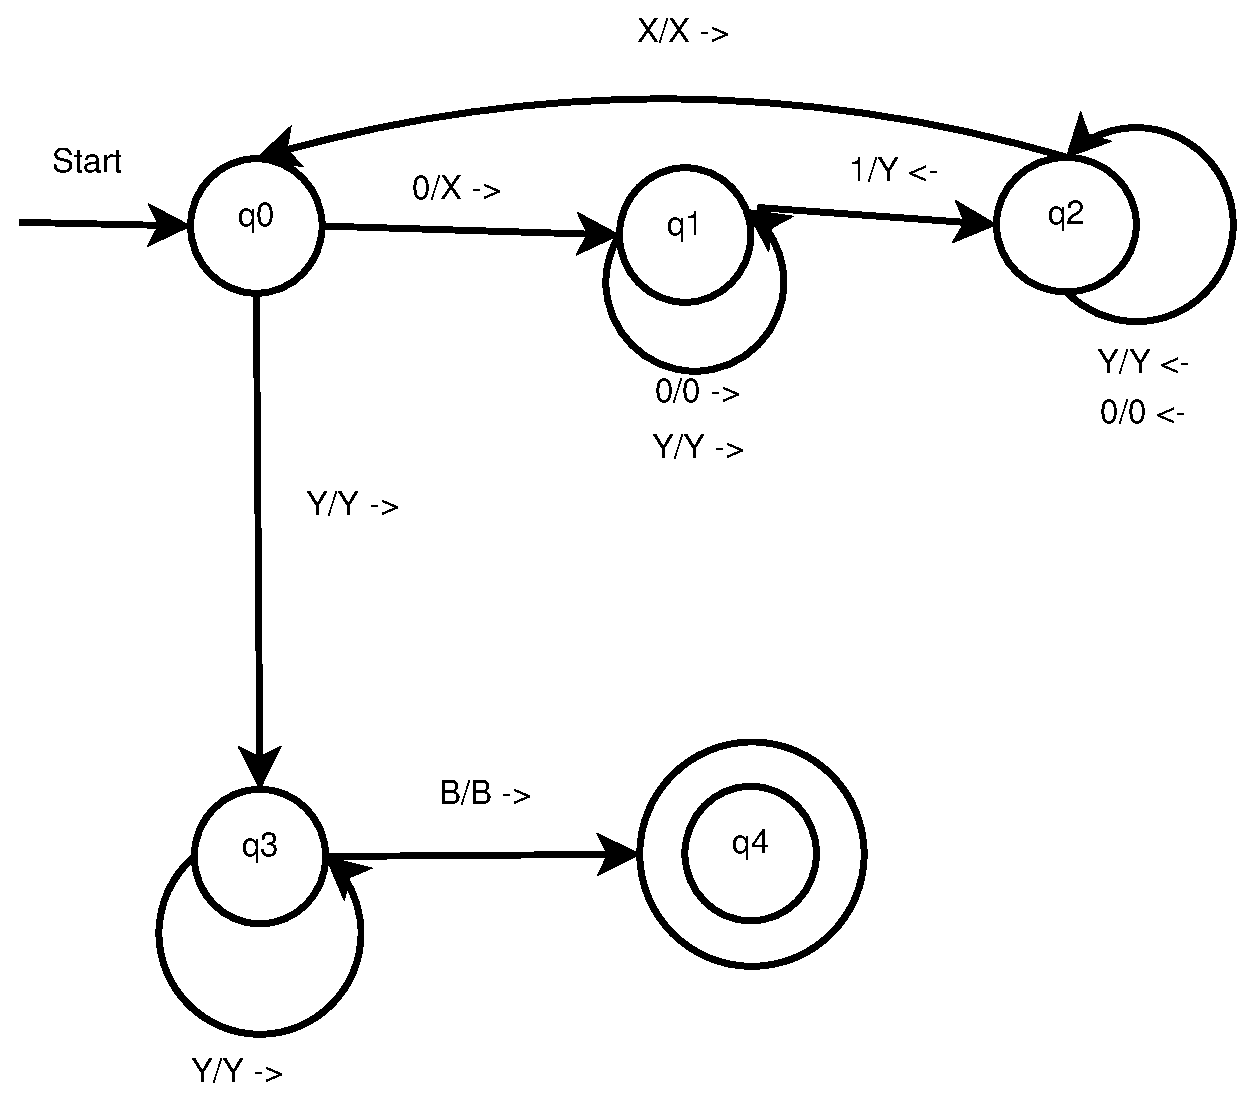
\includegraphics[scale=0.7]{tm}
\caption{接受形如$0^n1^n$的串的$TM$转移图}
\end{figure}

现在的问题就是-----对于任意的语言我们都能找到一个图灵机来为我们检验一个串是否属于这个语言么?

证明的思路就是假设某个这样的图灵机$M$存在,然后把其自身作为输入,输入给它自己,导出悖论,
从而否定其存在性。注意,否定了$M$的存在就是否定了这种判定方法的存在,也就否定了
这种算法的存在,也就否定了可判定问题。

要使图灵机能够接受自己作为输入,我们采用的策略是给图灵机进行编码,
使得每一个图灵机至少都有一个与之对应的字符串,为了简单起见,我们用
$0$和$1$对图灵机进行编码。

\begin{enumerate}
\item 首先确定所有$01$串的排序-----用字典序。即空串排在最前面,其余的串按长度排序,等长的字符串按位比较,$0$在$1$前面。
\item
\end{enumerate}

\chapter{Labmda演算}



%\chapter{函数式编程}

%\chapter{Why and Why NOT Lisp?}

\begin{thebibliography}{99}
\bibitem{face} 玑衡,面对面的办公室-----纪念艾伦•图灵百年诞辰.豆瓣网(2012)
\bibitem{tenth} 卢昌海,Hilbert第十问题漫谈(上).卢昌海的个人主页(2005)
\bibitem{dream} 方弦,希尔伯特之梦,以及梦的破灭.科学松鼠会(2009)
\bibitem{ialc} John E. Hopcroft,自动机理论、语言和计算导论.2008,215-286.
\end{thebibliography}

\end{document}
